\documentclass[12pt]{report}

\usepackage[utf8x]{inputenc}
\usepackage[T1]{fontenc}
\usepackage[frenchb]{babel}
\usepackage{lmodern}

\usepackage{amsmath,amsthm,amssymb}
\usepackage{graphicx}
\usepackage[colorinlistoftodos]{todonotes}
\usepackage{listings}
\usepackage{color}
\usepackage{verbatim}
\usepackage{grffile}


\definecolor{mygreen}{rgb}{0,0.6,0}
\definecolor{mygray}{rgb}{0.5,0.5,0.5}
\definecolor{mymauve}{rgb}{0.58,0,0.82}
\definecolor{darkWhite}{rgb}{0.94,0.94,0.94}

\lstset{
	aboveskip=3mm,
	belowskip=-2mm,
	backgroundcolor=\color{darkWhite},
	basicstyle=\footnotesize,
	breakatwhitespace=false,
	breaklines=true,
	captionpos=b,
	commentstyle=\color{red},
	deletekeywords={...},
	escapeinside={\%*}{*)},
	extendedchars=true,
	framexleftmargin=16pt,
	framextopmargin=3pt,
	framexbottommargin=6pt,
	frame=tb,
	keepspaces=true,
	keywordstyle=\color{blue},
	language=C,
	literate=
	{²}{{\textsuperscript{2}}}1
	{⁴}{{\textsuperscript{4}}}1
	{⁶}{{\textsuperscript{6}}}1
	{⁸}{{\textsuperscript{8}}}1
	{€}{{\euro{}}}1
	{é}{{\'e}}1
	{è}{{\`{e}}}1
	{ê}{{\^{e}}}1
	{ë}{{\¨{e}}}1
	{É}{{\'{E}}}1
	{Ê}{{\^{E}}}1
	{û}{{\^{u}}}1
	{ù}{{\`{u}}}1
	{â}{{\^{a}}}1
	{à}{{\`{a}}}1
	{á}{{\'{a}}}1
	{ã}{{\~{a}}}1
	{Á}{{\'{A}}}1
	{Â}{{\^{A}}}1
	{Ã}{{\~{A}}}1
	{ç}{{\c{c}}}1
	{Ç}{{\c{C}}}1
	{õ}{{\~{o}}}1
	{ó}{{\'{o}}}1
	{ô}{{\^{o}}}1
	{Õ}{{\~{O}}}1
	{Ó}{{\'{O}}}1
	{Ô}{{\^{O}}}1
	{î}{{\^{i}}}1
	{Î}{{\^{I}}}1
	{í}{{\'{i}}}1
	{Í}{{\~{Í}}}1,
	morekeywords={*,...},
	numbers=left,
	numbersep=10pt,
	numberstyle=\tiny\color{black},
	rulecolor=\color{black},
	showspaces=false,
	showstringspaces=false,
	showtabs=false,
	stepnumber=1,
	stringstyle=\color{gray},
	tabsize=4,
	title=\lstname,
}

\newtheorem{theo}{Théorème}[section]

\begin{document}

\begin{titlepage}

\newcommand{\HRule}{\rule{\linewidth}{0.5mm}} % Defines a new command for the horizontal lines, change thickness here

\begin{figure}
	\begin{minipage}[t]{.5\linewidth}
	\centering
	
\includegraphics[scale=0.5]{esilv_logo.png}\\[1cm]
	\end{minipage}
	\begin{minipage}[t]{.5\linewidth}
	
\includegraphics[scale=1.4]{edf_logo.png}\\[1cm]
	\end{minipage}
\end{figure}

\center % Center everything on the page


%	TITLE SECTION
%----------------------------------------------------------------------------------------

\HRule \\[0.4cm]
{ \huge \bfseries Pricer efficace d'actifs énergétiques}\\[0.4cm] % Title of your document
\HRule \\[1.5cm]

%----------------------------------------------------------------------------------------
%	AUTHOR SECTION
%----------------------------------------------------------------------------------------

\begin{minipage}{0.4\textwidth}
	\begin{flushleft} \large
		\emph{Team 16:}\\
		Anthony \textsc{Courillon} % Your name
		\\
		Denis \textsc{Barranco}
		\\
		Ousman \textsc{Asadullah}
		\\
		Hicham \textsc{Kortbi} % Your name
	\end{flushleft}
\end{minipage}
~
\begin{minipage}{0.4\textwidth}
	\begin{flushright} \large
		\emph{Partenaire:} \\
		Arnaud \textsc{de latour} % Supervisor's Name
		\\
		\emph{Mentor:} \\
		Martino \textsc{Grasselli} % Supervisor's Name
	\end{flushright}
\end{minipage}\\[2cm]

%----------------------------------------------------------------------------------------
%	DATE SECTION
%----------------------------------------------------------------------------------------

{\large Mars 2017}\\[2cm] % Date, change the \today to a set date if you want to be precise

\end{titlepage}


\chapter*{Introduction}
\addcontentsline{toc}{chapter}{Introduction}

Etant étudiants en quatrième année à l’ESILV dans la majeure finance et
dans le cadre du projet PI2, nous avons décidé de travailler sur la
réalisation d’un pricer d’actifs énergétiques proposé par notre partenaire EDF R\&D et encadré par Arnaud DE LATOUR

Un certain nombre d'actifs utilisés dans le domaine de l'énergie (par exemple les
centrales électriques) se prête facilement à une valorisation sous la forme de
produits dérivés complexes, de nature américaine (contrairement à une option
européenne, l'option américaine peut être exercée n'importe quand).

Le pricing de ces actifs met en oeuvre des méthodes numériques avancées qui
peuvent être coûteuses en temps de calcul. Lorsque ces méthodes sont fondées sur
une simulation Monte-Carlo (par exemple l'algorithme de Longstaff-Schwartz), on a
intérêt à employer des techniques de réduction de variance pour accélérer la
convergence de l'algorithme - et donc réduire le temps de calcul.

Cependant, l'efficacité de ces techniques dépend généralement du payoff de l'actif
qu'on cherche à valoriser. L'objectif de ce projet est donc d'implémenter et de
tester différentes méthodes de réduction de variance appliquées à des actifs
énergétiques, afin d'identifier les méthodes les plus pertinentes.

Nous allons réaliser ce pricer soous Python et nous allons utiliser exclusivement
ces 3 logiciels afin de réaliser ce projet:
\begin{itemize}
	\item Anaconda ;
	\item LiClipse ;
	\item Github.
\end{itemize}

\chapter{Evaluation du prix d'un produit dérivé par simulation}

\section{Principes des méthodes de Monte Carlo}

Le prix d'un produit dérivé d'un sous-jacent $X=(X_t)_{t\geq0}$ de payoff actualisé f(X), d'un marché financier sous probabilité risque neutre, s’écrit
comme l’espérance des flux futurs actualisés qu’il génère, $e_p$ :
\begin{equation}
	e_p = \mathbb{E}[f(X)]
\end{equation}
Il faut donc évaluer cette espérance pour connaître le prix d’un produit dérivé.
Nous allons utilize les méthodes de Monte Carlo qui consiste à simuler un grand
nombre de realisations, N indépendantes et identiquements distribuées, de f(X),
$f(X^i)$ avec $i\in \mathbb{N}$, puis on calcule chaque $f(X^i)$.

Enfin, on prend la moyenne empirique de ces réalisations, $\bar{e_N}$ estimateur de $e_p$ :
\begin{equation}
	\bar{e_N}=\frac{1}{N}\sum_{i=1}^{N} f(X^i) \xrightarrow[N\rightarrow{\infty}]{\text{p.s}} e_p \text{~avec~} \mathbb{E}[|f(X)|]<\infty
\end{equation}
la loi des grand nombres assure la convergence de $\bar{e_N}$ vers $e_p$.
Autrement dit, pour N assez grand, $\bar{e_N} \simeq e_p$.

\section{Limite pratique des méthodes de Monte Carlo}

\begin{theo}[Théorème Central Limite]\label{TCL}
	Nous allons utilisé le cas où on ne connait pas la loi de $e_p$.
	Si la loi de $e_p$ est inconnue (ou non normale), alors $\bar{e_N}\hookrightarrow N(\mu,\frac{\sigma}{\sqrt{N}})$ pour N assez grand, avec $\sigma$ = $\sqrt{(Var(f(X)))}$  et $\mu=e_p =\mathbb{E}[f(X)]$  alors on a:
	\begin{equation}
		\frac{\sqrt{N}(\bar{X}_n-\mu)}{\sigma}\hookrightarrow N(0,1)
	\end{equation}
\end{theo}

Donc le théorème central limite permet d'avoir l'approximation de l'erreur réalisée:
\begin{equation}
	\label{eq:approximation-erreur}
	\sqrt{N}(\frac{1}{N}\sum_{i=1}^{N}f(X^i)-e_p)\hookrightarrow N(0,\sqrt{Var(f(X))})
\end{equation}
ou :
\begin{equation}
	\sqrt{N}(\bar{e_N}-e_p)\hookrightarrow N(0,\sqrt{Var(f(X))})
\end{equation}

Cela montre le problème du nombre de simulations N nécessaires pour avoir un bon estimateur de $e_p$, plus la variance de $f(X^i)$ est élevé, plus N doit être grand.

Or N grand a pour conséquence une augmentation du temps de calcul. Donc plus $Var(f(X^i))$, plus l’obtention de l’évaluation de $e_p$ demandera un temps de calcul important.

Il est alors intéressant d’employer des techniques de réduction de variance pour accélérer la convergence de l’algorithme et donc réduire le temps de calcul. C’est l’un des problèmes que nous allons tenter de résoudre dans la réalisation de notre pricer.

Nous allons voir les différentes techniques de réduction de variance et tenter de les implémenter dans notre pricer dans le chapitre 2 de ce document.

\section{Contrôle de la convergence}

Il faut évaluer l’erreur d’approximation de \eqref{eq:approximation-erreur}  grâce à la construction d’un intervalle de confiance :
\begin{equation}
	Z = \frac{\sqrt{N}}{\sqrt{Var(f(X))}} (\frac{1}{N}\sum_{i=1}^{N}f(X^i)-e_p)\hookrightarrow N(0,1)
\end{equation}
En supposant que la variance est connue, on a :
\begin{equation}
	\mathbb{P}(-u\leq Z \leq u) = \alpha
\end{equation}
avec u fractile d'ordre 1-$\frac{\alpha}{2}$ de la N(0,1). Ce qui revient à :
\begin{equation}
	\mathbb{P}(-u \frac{\sqrt{Var(f(X))}}{\sqrt{N}}+\bar{e_N}\leq e_p \leq u \frac{\sqrt{Var(f(X))}}{\sqrt{N}}+\bar{e_N}) = \alpha
\end{equation}
et donc :
\begin{equation}
	\text{IC}_\alpha(e_p) = [-u \frac{\sqrt{Var(f(X))}}{\sqrt{N}}+\bar{e_N};u \frac{\sqrt{Var(f(X))}}{\sqrt{N}}+\bar{e_N}]
\end{equation}
L’erreur donné par un intervalle de confiance est :
\begin{equation}
	\mathbb{P}(e_p\in IC_\alpha ) \simeq \alpha
\end{equation}
Il a un problème c’est qu’on ne peut appliquer cette méthode que si la variance de f(X), Var(f(X)) est connue. Or ici, Var(f(X)) est inconnue, et il faut l’estimer grâce à un estimateur.

On peut construire un estimateur non biaisé tel que celui-ci :
\begin{equation}
	\bar{v_N} = \sqrt{\frac{1}{N-1}\sum_{i=1}^{N}(f(X^i)-\bar{e_N})^2}
\end{equation}

Voici l’implémentation sous Python de tout ce que nous avons énoncé dans cette partie I, on a pris  $\alpha$ =0.95 pour la contruction des intervalles de confiance.
\begin{lstlisting}
class GaussianGenerator:
"Générateur de bruits gaussiens corrélés."

def __init__(self, nsims, corrmatrix, corrkeys, randomfunc):
"""
Initialise une nouvelle instance de la classe `GaussianGenerator`.

Paramètres :
------------
nsims : entier positif
Nombre de simulations à générer.
corrmatrix : matrice carrée
Matrice de corrélation entre les différents bruits gaussiens
à simuler. La matrice doit être définie positive.
corrkeys
Liste des identifiants associés aux différentes lignes / colonnes
de la matrice de corrélation `corrmatrix`. Les identifiants doivent
être donnés dans l'ordre dans lequel les bruits correspondants
apparaissent dans `corrmatrix`.
randomfunc
Fonction permettant de générer des bruits gaussiens indépendants
(typiquement `np.random.randn`).
"""
self.corrmatrix = corrmatrix
self.corrkeys = corrkeys
self.nsims = nsims
self.randomfunc = randomfunc
self.cache = DateCache()
try:
np.linalg.cholesky(self.corrmatrix)
except np.linalg.LinAlgError:
raise np.linalg.LinAlgError("the correlation matrix is not "\
"positive definite.") from None

@property
def nnoises(self):
"Nombre de bruits gaussiens distincts à simuler."
return self.corrmatrix.shape[0]

@timecached
def getallnoises(self, date):
"""
Renvoie `self.nsims` réalisations de `self.nnoises` bruits
gaussiens corrélés.
"""
whitenoises = self.randomfunc(self.nnoises, self.nsims)
noises = np.dot(np.linalg.cholesky(self.corrmatrix), whitenoises)
return noises

@timecached
def getnoises(self, date, keys):
"""
Renvoie un tableau de taille `(len(keys), self.nsims)` de bruits
gaussiens corrélés correspondants aux aléas identifiés par les
clefs `keys`.
"""
noises = self.getallnoises(date)
res = np.empty((len(keys), self.nsims))
for idx, key in enumerate(keys):
keyidx = self.corrkeys.index(key)
res[idx, :] = noises[keyidx, :]
return res

\end{lstlisting}

\chapter{Méthodes de réduction de la variance}
\section{Variables antitthétiques}
L’idée des variables antithétiques repose sur la symétrie de la
distribution de la loi uniforme et la correlation entre 2
variables aléatoires.
\subsection{Idées globales}
Calculer $\theta$ = $\text{E}[Y]$=$\text{E}[f(X)]$\\
$\text{E}[Y]$=$\frac{1}{2}$$\text{E}[Y_1]+\text{E}[Y_2]=\text{E}[\frac{Y_1+Y_2}{2}]$\\
Var($\frac{Y_1+Y_2}{2})=\frac{Var(Y_1)+Var(Y_2)+2Cov(Y_1,Y_2)}{4}$\\
- Si $Y_1$ et $Y_2$ sont indépendantes, Cov($Y_1,Y_2$)=0\\
-Si Cov($Y_1,Y_2$)<0, alors $Var(\frac{Y_1+Y_2}{2})<Var(\frac{Y}{2})$ donc la variante est réduite si $Y_1$ et $Y_2$ sont corrélés négativements, Cov($Y_1,Y_2)<$0\\\\
\subsection{Mathématiquement}
On veut estimer $\text{E}[Y]$ en utilisant l'implémentation d'échantillons antithétiques c'est-à-dire: $(Y_1,Y_{1ant}),(Y_2,Y_{2ant}),...,(Y_N,Y_{Nant})$  avec $\forall$ i $\in$ $\mathbb{N}$, $Y_i$ et $Y_{iant}$ de même loi de distribution et i.i.d. (indépendantes et identiquement distribuées).\\
L'estimateur de $\text{E}[Y]$ est simplement la moyene des 2N réalisations:\\\\
$\bar{e_{Nant}}$=$\frac{1}{2N}(\sum_{i=1}^{N}Y_i +\sum_{i=1}^{N}Y_{iant})$=$\frac{1}{N}\sum_{i=1}^{N}(\frac{Y_i+Y_{iant}}{2})$\\\\
En utilisant les mêmes méthodes que dans le chapitre I, on par TCL:\\
\begin{center}
	$\frac{\sqrt{N}(\bar{e}_{Nant}-\text{E}[Y])}{\sqrt{Var(Y)}}$
\end{center}
On pose $\sigma^2_{ant}=Var(Y)=Var(\frac{Y_i+Y_{iant}}{2})$\\\\
Comme nous venons de le voir dans les idées globales:\\\\
$\sigma^2_{ant}=\frac{Var(Y_i)+Var(Y_{iant})+2Cov(Y_i,Y_{iant})}{4}$\\\\
$ =\frac{2Var(Y_i)+2Cov(Y_i,Y_{iant})}{4}$ car $Y_i $ et $ Y_{iant}$ sont de même loi de distribution\\\\
$=\frac{Var(Y_i)+2Cov(Y_i,Y_{iant})}{2}$\\\\
Alors, si $Cov(Y_i,Y_{iant}) <0$, $\sigma^2<\frac{Var(Y_i)}{2}$\\\\
Donc nous avons besoin de construire les paires $Y_i$ et $Y_{iant}$ de façon à ce que $Cov(Y_i,Y_{iant}) <0$ pour réduire la variance.\\\\
\subsection{Implémentation}
Comme nous simulons une matrice de bruits gaussiens indépendants, on peut implémenter la méthode des variables antithétiques en construisant une séquence $Y_i,Y_2,...,Y_N$ (rappel: $f(X^i)$ avec i $\in \mathbb{N})$ puis construire une autre séquence opposé à la première en prenant la négation de celle-ci: $-Y_1,-Y_2,...,-Y_N.$\\\\
Pseudo-code:\\
1. Créer une matrice vide de taille (nnoises,nsims) avec \\nnoises: nombre de bruits gaussiens indépendants \\ nsims: nombre de simulations\\
2. Générer dans la moitié de la matrice des bruits gaussiens.\\
3. Prendre l'opposé de la première moitié de la matrice, pour remplir la deuxième moitié de la matrice.\\\\
Voici l'implémentation sous Python de la méthode des variables antithétiques:
\begin{lstlisting}
def antithetic_randn(nnoises, nsims):
"""
Renvoie un tableau de bruits gaussiens non corrélés :math:`(G_{_i,j})`
de taille `(nnoises, nsims)`, et tel que, pour tout :math:`i` :
:math:`\forall 1 \leq j \leq n / 2, G_{i,n/2+j} = -G_{i,j}`

Paramètres :
------------
nnoises : entier positif
Nombre de bruits à simuler.
nsims : entier positif, pair
Nombre de simulations à effectuer par prix.
"""
if nsims % 2 != 0:
raise ValueError("the number of simulations used with antithetic "\
"variables should be even.")
half = int(0.5 * nsims)
noises = np.empty((nnoises,nsims))
noises[:, :half] = np.random.randn(nnoises, half)
noises[:, half:] = -noises[:, :half]
return noises

\end{lstlisting}
\newpage
\section{Suites à discrépance faible (Quasi Monte Carlo)}
Nous allons étudier les méthodes de Quasi Monte Carlo qui contrairement au Monte Carlo classique n'est pas basé sur la génération de nombres pseudo-aléatoires mais sur la génération de nombre déterministe aux propriétés spéciales générés par des suites à discrépance faible.//
On peut voir le problème de l'évaluation du prix d'un produit dérivé vu dans le chapitre I (1)  comme une intégrale à la place d'une espérance:\\\\
$e_p^{QMC}=$$\int_{[0,1]^s} f(u) \, \mathrm du$=$\frac{1}{N}\sum_{i=1}^{N}f(X^i)$\\\\
On cherche à approximer l'intégrale.\\
Pour cela, il faut générer les points $X^i$ dans l'hypercube $[0,1]^s$ avec s la dimension de l'espace.
Ces points doivent être équiréparties.
On ne se souciait pas vraiment de la dimension jusqu'à présent mais plus la dimension sera grande, plus il y aura des irrégularités dans les projections.\\
Nous allons voir les différentes suites à discrépance faible permettant de générer ces points.


Discrépance et propriétés d'équirépartition à détailler.(a faire)
\subsection{Suite de Van Der Corput}

La suite de Van der Corput en base b est de la forme:\\
$\phi_b(n)=\frac{a_o}{b}+\frac{a_1}{b^2}+...+\frac{a_r}{b^{r+1}}$\\ avec n=$a_0+a_1+...+a_rb^r$, $a_r>0$, $0\leq a_i \leq p$, $0\leq i \leq r$
\begin{center}
	ou \\
\end{center}
$\phi_b: \mathbb{N} \rightarrow[0,1)$]\\
$\forall$ $ b\in \mathbb{N}$, $\phi_b(n)=\sum_{i=0}^{\infty}\frac{a_i(n,b)}{b^{i-1}}$\\\\

Nous allons voir les suites de Van Der Corput avec deux exemples ayant chacun leur approche. C'est important de bien comprendre cette suite car elle est la clé de la compréhension des suites qui vont suivre.\\\\

\subsubsection{Exemple 1: l'approche classique}
Nous allons prendre un exemple d'une suite de Van Der Corput en base 2 distribué sur l'intervalle [0,1).\\
Pour n=12, les nombres générés sont: 0,$\frac{1}{2},\frac{1}{4},\frac{3}{4},\frac{1}{8},\frac{5}{8},\frac{3}{8},\frac{7}{8},\frac{1}{16},\frac{9}{16},\frac{5}{16},\frac{13}{16}$\\
\bigbreak
\begin{figure}[h]
	\begin{center}
	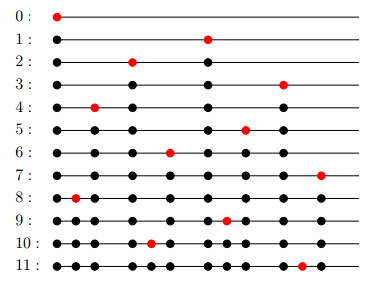
\includegraphics[scale=0.5]{figure1-van-der-corput.png}\\
	\end{center}
\caption{Suite de Van Der Corput en base 2 pour n=12}
\end{figure}
Les nombres générés séquentiellement remplissent les larges espaces entre les nombres précédents de la séquence.\\
\\En prenant la logique de la construction d'une suite de Van Der Corput, nous avons implémenté sous Python les fonctions permmettant de générer la séquence:\\
\begin{lstlisting}
def vdc(n, base):
"""
Cette fonction permet de calculer le n-ieme nombre de la base b de la 
séquence de Van Der Corput
"""
vdc, denom = 0,1
while n:
denom *= base
n, remainder = divmod(n, base)
vdc += remainder / denom
return vdc
\end{lstlisting}
\bigbreak

\begin{lstlisting}
def van_der_corput(nsims,b):
"""
Cette fonction permet de générer la séquence de Van Der Corput en base b
"""
array=np.empty(nsims)
i=0
for i in range(nsims):
array[i]=vdc(i,b)
return array
\end{lstlisting}
On a testé ces fonctions et on a tracé ceci:\\
\begin{figure}[h]
	\begin{center}
		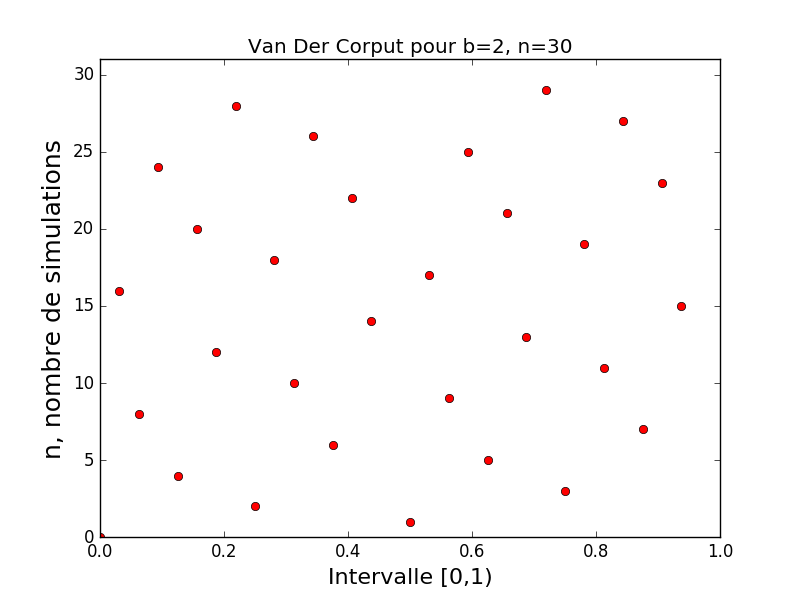
\includegraphics[scale=0.5]{figure_1-van_der_corput_exemple1.png}\\
	\end{center}
	\caption{Suite de Van Der Corput en base 2 pour n=30}
\end{figure}
\medbreak
On voit bien sur la figure 2.2 que le points générés par la séquence de Van Der Corput sont plutôt bien équiréparties.
\subsubsection{Exemple 2:l'approche binaire}
On peut calculer le n-ième terme de la suite de Van Der Corput de base b comme ceci: ( à expliquer plus en détails)
\begin{figure}[h]
	\begin{center}
		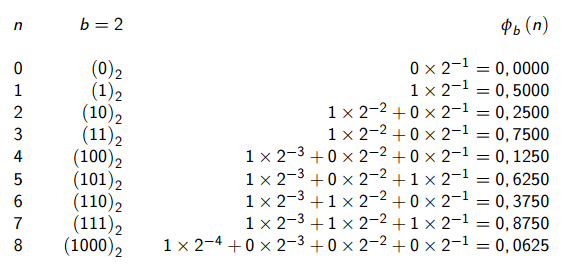
\includegraphics[scale=0.5]{figure2.3-van_der_corput_binaire.png}\\
	\end{center}
	\caption{Suite de Van Der Corput en base 2 pour n=30}
\end{figure}
\subsubsection{Implémentation de la suite de Van Der Corput}
Voici l'implémentation sous Python.\\
remarque: comme la suite de Van Der Corput génère des points dans l'intervalle [0,1), il a fallu modifier la fonction vdc (sans cette modification, on n'obtenait pas des résultats ce rapprochant du Monte Carlo classique) en prenant l'inverse de la CDF(cumulative distribution function), à vérifier
\begin{lstlisting}
	def vdc(n, base):
	"""
	Cette fonction permet de calculer le n-ieme nombre de la base b de la 
	séquence de Van Der Corput
	"""
	vdc, denom = 0,1
	while n:
	denom *= base
	n, remainder = divmod(n, base)
	vdc += remainder / denom
	return norm.ppf(vdc)
	
	def van_der_corput(nsims,b):
	"""
	Cette fonction permet de générer la séquence de Van Der Corput en base b
	"""
	array=np.empty(nsims)
	i=0
	for i in range(nsims):
	array[i]=vdc(i,b)
	return array
	
	def van_der_corput_dimension(dim,nsims):
	array=np.empty((dim,nsims))
	"""
	Cette fonction génère dans un tableau de taille (dim,nsims) toutes les séquences
	de la suite de Van der Corput de la base 2 à la base dim+2
	"""
	for i in range(2,dim+2,1):
	array[i-2,:]=van_der_corput(nsims, i)
	return array
	
\end{lstlisting}

\subsection{Suite de Sobol}
Explication de la suite de Sobol à faire
\begin{lstlisting}
import sobol_seq

def sobol(nnoises,nsims):
"""
Renvoie un tableau de valeurs générés par la suite de Sobol
de taille (nnoises,nsims)
"""
noises = np.empty((nsims))
"""
Utilisation de la fonction sobol_seq.i4_sobol_generate_std_normal
pour générer des variables quasi-aléatoires suivant une loi normale
"""
noises=sobol_seq.i4_sobol_generate_std_normal(nnoises,nsims)
return (noises.reshape(nnoises,nsims))

\end{lstlisting}
\end{document}
